\documentclass[a4paper]{report}
\usepackage[utf8]{inputenc}
\usepackage[T1]{fontenc}
\usepackage{listings}
\usepackage{graphicx}

\usepackage{amsmath,amsfonts,amssymb,amsthm}
\usepackage{listings,graphicx,caption}
\usepackage{epstopdf}
\usepackage{etoolbox,xcolor,titlesec,bm,tabularx}
\definecolor{light-gray}{RGB}{231,255,231}
\definecolor{light-blue}{RGB}{245,245,255}
\definecolor{light-yellow}{RGB}{245,245,245}
\usepackage{graphicx}
\usepackage{caption}
\usepackage{float}
\usepackage{geometry}
\usepackage{listings}
\usepackage{enumerate}
\usepackage{enumitem}
\usepackage{float}
\usepackage{epstopdf}
\geometry{hmargin=1.5cm,vmargin=2.5cm}
\lstset{language=Matlab,breaklines=true, frame = single,keywordstyle=\color{blue},morekeywords=[2]{1}, keywordstyle=[2]{\color{black}},
identifierstyle=\color{orange},stringstyle=\color{magenta},commentstyle=\color{green},showstringspaces=false,numbers=left,numberstyle={\color{gray}},
numbersep=10pt}

\title{ Solving Stochastic PDE's   }
\author{Oxana USHAKOVA}
\date {\today}
\begin{document}
\maketitle
\tableofcontents
\newpage
\section*{Notations}
\begin{itemize}
\item $S$ - Stock price, also called Spot price (or any underlying asset)
\item $V(S,t)$ - value of an option, depending on time and spot price
\item $K$ - Strike price
\item $r$ - risk-free rate
\item $d$ - dividend yield
\item $\mu$ - drift rate of $S$ - the rate at which the average of $S$ changes
\item $\sigma$ - volatility of the stock, standard deviation of $log(S)$ - return on stock
\item $T_0$,$T$ - initial and final time
\item $\theta$ - long variance : as $t$ tends to infinity, the expected value of $\nu$ tends to $\theta$ 
\item $\kappa$ - the rate at which $\nu$ reverts to $\theta$
\item $\xi$ - the volatility of volatility
\end{itemize}


\newpage
\section*{Introduction}


The main objective of this project is to learn what are stochastic PDE's and how to solve them. As PDE we took the Black-Scholes model widely used in finance. 
\newline
The paper can be divided in 5 parts. Firstly, we give some basic concepts in finance and stochastic calculus. Then we focus on Black-Scholes model, its derivation and analytical solution. In two last chapters we implement finite elements method and finite difference method in FreeFem++, Feel++, C++. Some of plots are made in Octave, Java and gnuplot(C++). We want to compare those methods and find the most suitable way to price a financial instrument.

  

\chapter{Financial Market : basics}





Computational finance is an interdisciplinary field which joins financial mathematics, stochastic calculus, numerics and scientific computing. Its goal is to estimate as accurately and efficiently as possible the risks that financial instruments generate. In this project we will focus on options.
\begin{figure}[H]
    \centering
    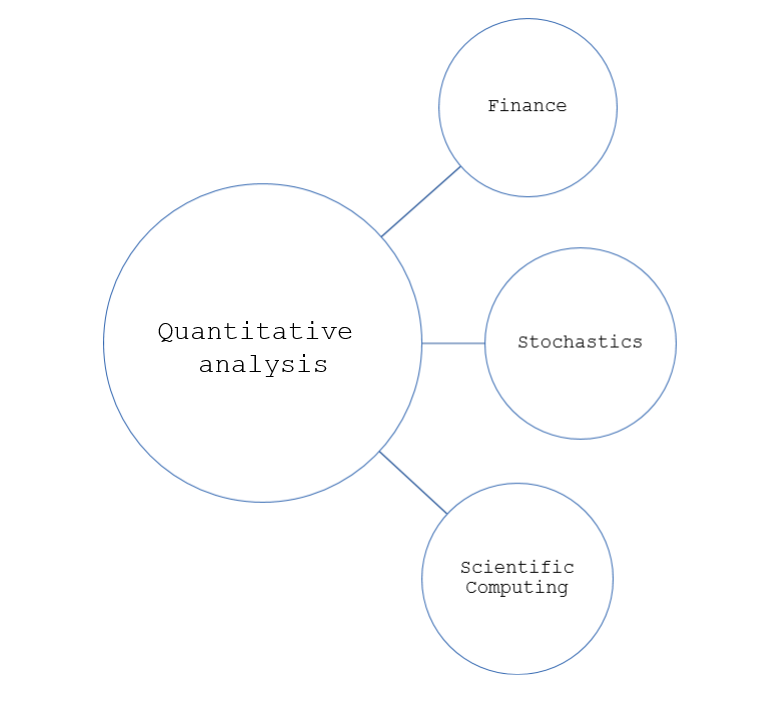
\includegraphics[width=0.5\textwidth]{dia.png}
    \caption{Financial mathematics}
\end{figure}


\section{Option as a financial instrument}

An \textbf {Option} is a contract that gives the buyer the right,\textit{  but not the obligation}, to buy or sell an underlying asset (a stock, a bond, gold, other option, etc.) at a specific price, called \textbf{ Strike} price, on or before a certain date. An option is a security, just as stokes or bonds, it has its own price called \textbf {Premium}.
\\
\\
Every option contract has several parameters to
be pre-set at $t=T_0$ :
\begin{itemize}
\item Who buys (long), who sells (short)?
\item What is the underlying asset ?
\item What is the maturity $T$ of the contract ?
\item Does the contract give the right to buy (\textbf{call option}) or to sell(\textbf{put option}) ?
\item What is the Strike price $K$ ?
\item What is the price of the option itself, i.e. premium?

Obviously, the asymmetry of the option contract leads us to the question if we buy this contract it or we sell it. A buyer of an option contract is said to be in \textbf{long} positions, the seller - in \textbf{short} position.
\\
\\
Let's take a look on potential gain diagram for Long Call Option:
\\
\\
\begin{figure}[H]
    \centering
    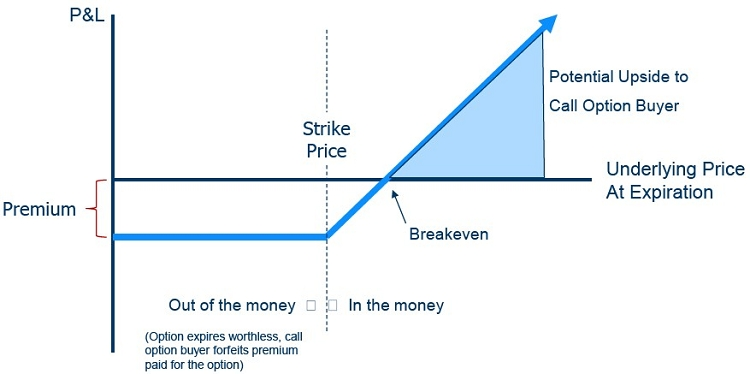
\includegraphics[width=0.8\textwidth]{payoff.png}
    \caption{Long Call Option}
\end{figure}


As it comes from the figure 1,  Long Call Option brings profit (« in the money ») , if $S$ at maturity $T$ is higher than the breakeven point. So the payoff of this option is premium ignored):
\begin{itemize}
\item[$\bullet$]  $S - K$ if $S(T)>K$\\
\item[$\bullet$]  $0$ if $S(T)<K$\\
\end{itemize}
Here are all 4 possible payoffs:
\begin{figure}[H]
    \centering
    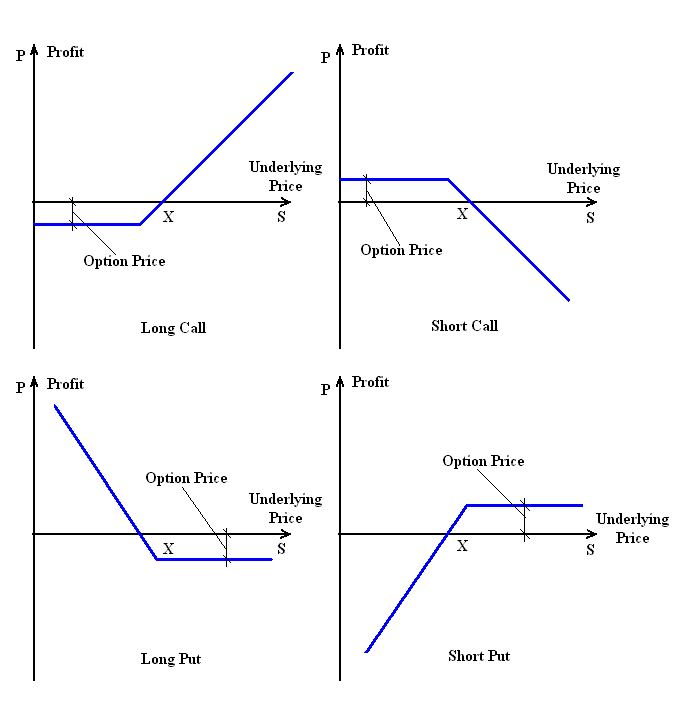
\includegraphics[width=0.7\textwidth]{OptionsProfit.png}
    \caption{Possible payoffs}

\end{figure}




\subsection{Put-Call Parity}

The put–call parity defines a relationship between the price of a European call option and European put option, both with the identical strike price and maturity.\\
We consider two portfolios:

\begin{itemize}
\item {one European call ($C$) and cash ($Ke^{-rT}$)}
\item {one European put ($P$) and one share ($S_0$)}
\end{itemize}

At time $T$ they both worth $max(S_T, K)$, hence their values should be equal today, i.e.:
\begin{equation}
C + Ke^{-rT} = P + S_0
\end{equation}

\subsection{Vanilla vs Exotics}


This type of of options is said to be \textbf{Vanilla} : the simplest version of all, without any optional extras, by analogy with the default ice cream flavour, vanilla. There exist a rich family of, so called \textbf{Exotic} options. Here we list only several of them:
\begin{itemize}
\item American option (Bermuda)
\\can be executed not only at $T$,but on any time of life of the option $(T_0,T)$;
\\Bermuda option can be executed on a specific period during the life of the option, i.e. every second Monday, June, etc.
\item Barrier option (Paris)
\\can be activated for be executed only if the asset price touches (or not) a specific barrier;
\\Paris barrier option can be activated for be executed only if the asset price satisfy the barrier condition for a certain period of time (i.e. 15min, 1 day, 30\%, etc).
\item Asian option
\\its payoff is determined by the average underlying price over some pre-set period of time.
\item Lookback option (Russian)
\\its payoff depends not at $S$ at final time $T$, $S(T)$, but on $max(S)$ over the life of the option.
\\Russian lookback option is a special case of lookback : it has no pre-set expiration time, it's up to buyer of the option when to execute it. It's also called 'no regret' option. 
\end{itemize}



\section{Option Pricing models}

\subsection{Pricing Models}



\begin{figure}[H]
    \centering
    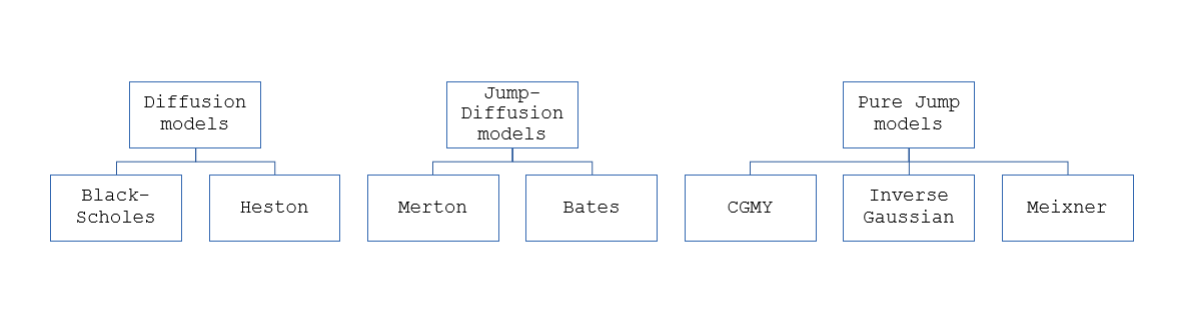
\includegraphics[width=\textwidth]{models.png}
\end{figure}


\begin{itemize}
\item[$\bullet$] \textbf{Diffusion models} have only a diffusion component, given by Wiener process : \textit{Black-Scholes, Heston};\\
\begin{itemize}


\item  Black-Scholes model\\
$ dS=\mu S dt + \sigma S dB$\\
$B$, and consequently its increment $dB$,represents the only source of 'diffusion' uncertainty in the price history of the stock.\\


\item Heston model \\
$ dS=\mu S dt + \sqrt{\nu} S dB$\\
$ d\nu = \kappa(\theta-\nu)dt +\xi\sqrt{\nu}dB$\\
$B$, and consequently its increment $dB$, and $\nu$, and consequently root from it, represent two sources of 'diffusion' uncertainty in the price history of the stock.\\
\end{itemize}


\item[$\bullet$] \textbf{Jump diffusion models}  have both diffusion component, given by Wiener process, and jump component, given by compounded Poisson process : \\
\\
\textbf{Rq:} For financial applications, it is of little interest to have a process with a single possible jump size. The compound Poisson process is a generalization where the waiting times between jumps are exponential but the jump sizes can have an arbitrary distribution.
\\
\begin{itemize}
\item Merton model\\
$ dS=\mu S dt + \sigma S dB + \sum_{n=1}^{N_t} Y_i$\\
$dB$ represents the source of 'diffusion' uncertainty and the last term represents is the source of 'jump' uncertainty (compound Poisson process with Gaussian jumps) in the price history of the stock. $dB$ and $\nu$ represent the source of 'diffusion' uncertainty and the last term represents is the source of 'jump' uncertainty (compound Poisson process with Gaussian jumps) in the price history of the stock.\\
It mixes Black-Scholes model Compounded Poisson process.\\

\item Bates model\\
$ dS=\mu S dt + \sqrt{\nu} S dB + \sum_{n=1}^{N_t} Y_i$ \\
$ d\nu = \kappa(\theta-\nu)dt +\xi\sqrt{\nu}dB$\\

$dB$ and $\nu$ represent the source of 'diffusion' uncertainty and the last term represents is the source of 'jump' uncertainty (compound Poisson process with Gaussian jumps) in the price history of the stock.\\
It mixes Merton and Heston models.\\

\end{itemize}

\item[$\bullet$] \textbf{Pure jump models} have no diffusion, just a random process : \\
\begin{itemize}
\item CGMY process
\item Inverse Gaussian Process
\item Meixner process
\item etc
\end{itemize}
\end{itemize}

\section{Greeks}
\textbf{Greeks} are the quantities representing the sensitivity of the price of
options to a change in underlying parameters. We list some of them, further in the project we will study them:
\begin{itemize}
\item \textbf{Delta} - the rate of change of the option price w.r.t. the price of the underlying asset:
\begin{equation}
\delta = \frac{\partial C}{\partial S}
\end{equation}
\item \textbf{Theta} - the rate of change of the portfolio price w.r.t. the time:
\begin{equation}
\theta = \frac{\partial \Pi}{\partial t}
\end{equation}
\item \textbf{Gamma} - the rate of change of the $\delta$  w.r.t. the price of the underlying asset:
\begin{equation}
\Gamma = \frac{\partial^2 \Pi}{\partial S^2}
\end{equation}
\item \textbf{Vega} - the rate of change of the portfolio price w.r.t. the volatility of the underlying asset:
\begin{equation}
\upsilon = \frac{\partial \Pi}{\partial \sigma}
\end{equation}
\item \textbf{Rho} - the rate of change of the portfolio price w.r.t. the interest rate:
\begin{equation}
\upsilon = \frac{\partial \Pi}{\partial r}
\end{equation}
\end{itemize}
Here are some graphical representations of what are Greeks:
\begin{figure}[H]
    \centering
    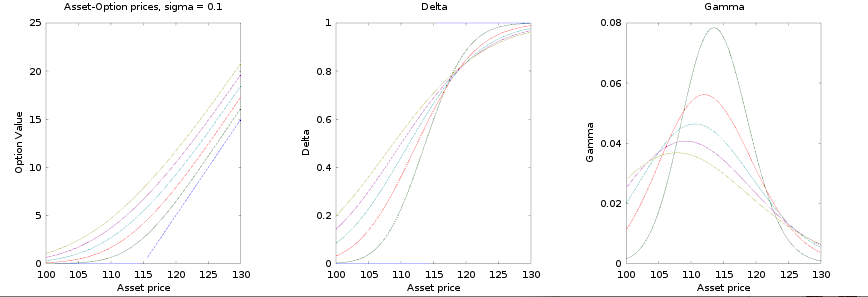
\includegraphics[width=\textwidth]{octave1.png}
    \caption{Delta and Gamma for $\sigma$ = 0.1 }
\end{figure}

\begin{figure}[H]
    \centering
    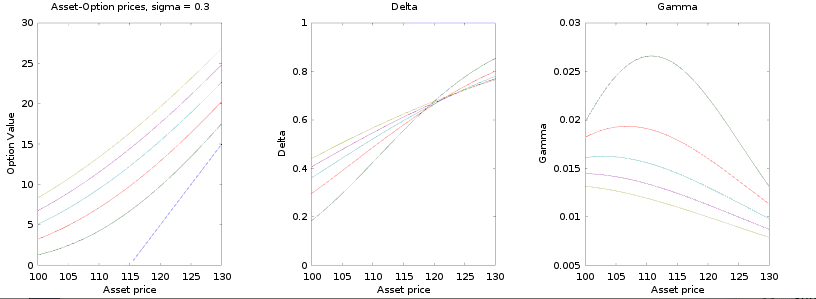
\includegraphics[width=\textwidth]{octave2.png}
    \caption{Delta and Gamma for $\sigma$ = 0.3}
\end{figure}

\begin{figure}[H]
    \left
    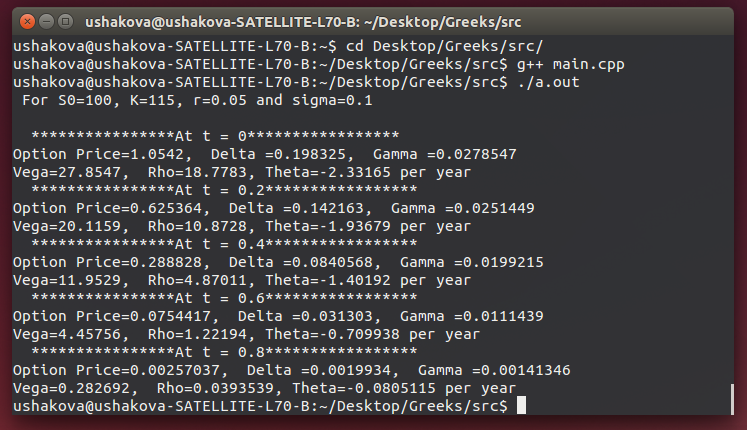
\includegraphics[width=0.7\textwidth]{gpp.png}
    \caption{ Greeks }
\end{figure}


\chapter{Stochastics : basics}
In this section we give concepts that will be used further when the existence and the uniqueness of a solution for a stochastic PDE will be discussed.

\section{Stochastic process}


A \textbf{stochastic process} in discrete time, denoted by $(X_t)_{t \in \mathcal{T}}$, is a sequence of random variables $X_0,X-1,..X_T$ defined on a probability space ($\Omega, \mathcal{A}, \mathbb{P}$) with values in $\mathbb{R}$. For a given $\omega \in \Omega$, the sequence $X_t(w), t\in \mathcal{T}$ is called a \textbf{path} of the process ($X_t$), where $\mathcal{T}$ stands for time series (dates) : $\mathcal{T}=\{0,1,..T\}$
\\

\section{ Filtrations}

A \textbf{filtration} $\mathcal{F}$ on a probability space  ($\Omega, \mathcal{A}, \mathbb{P}$) is a sequence of $\sigma$-algebras $\mathcal{F}_0 \subseteq \mathcal{F}_1 \subseteq ...  \subseteq \mathcal{F}_T \subseteq \mathcal{A}$. A quadruple ($\Omega, \mathcal{A}, \mathbb{P}, \mathcal{F})$ is called a \textbf{filtered probability space}.\\
A stochastic process $(X_t)_{t \in \mathcal{T}}$ is sais to be \textbf{adapted to a filtration} $\mathcal{F}$ if for all $t \in \mathcal{T}$, the random variable $X_t$ is $\mathcal{F}_t$ - measurable.\\

\section{ Martingales}

Let ($\Omega, \mathcal{A}, \mathbb{P}, \mathcal{F})$) be a filtered probability space. A stochastic process $X = (X_t)_{ t \in \mathcal{T}}$ is called a \textbf{martingale} if
\begin{enumerate}
\item $X$ is adapted to $\mathcal{F}$
\item $\mathbb{E} [|X_t|] < \inf \forall \in \mathcal{T}$
\item $\mathbb{E} [X_t|\mathcal{F}_s]=X_s \forall t \geq s$
\end{enumerate}
Note, the following brownian martingale is used in the Black-Scholes theory:
\begin{equation}
(e^{\alpha B_t - \frac{\alpha^2}{2}t})
\end{equation}
and 
\begin{equation}
\mathbb{E}[e^{\alpha B_t - \frac{\alpha^2}{2}t}|\mathcal{F_s} = e^{\alpha B_s - \frac{\alpha^2}{2}s}, 0 \leq s < t
\end{equation}

\section{Itô Calculus } 

The \textbf{Itô integral} is the central concept of Itô calculus. The integrand and the integrator  are  stochastic processes:
\begin{equation}
Y_t=\int_0^t X_s dB_s,
\end{equation}

where $X$ is a locally square integrable process adapted to the filtration generated by $B$, which is a Wiener process or Brownian motion. The result of the integration is another process.\\

If we assume that  $\{\pi_n\}$ is a sequence of partitions of $[0,t]$ with min mesh size, then the integration by parts for Itô integral is given by :
\newline
\newline
$\int_0^t XdB = \lim_{n\to\infty} \sum_{t_{i-1},t_i \in \pi_n} X_{t_{i-1}}(B_{t_i}-B_{t_{i-1}})$.
\newline
\newline
$X$ is square integrable, then its integral w.r.t. $B$ can be defined and $X$ is said to be $B$-integrable. As $\int_0^t (X-X_n)^2ds \rightarrow 0$ in probability, the Itô integral becomes:\\

$\int_0^tXdB=\lim_{n\to\infty} \int_0^t X_ndB$\\

where we faal again on convergence in probability. This leads us to a very important property: \textbf{Itô isometry}:\\
\begin{equation}
\mathbb{E}[(\int_0^t X_sdB_s)^2] = \mathbb{E}[\int_0^t X_s^2ds]
\end{equation}


\section{Itô's lemma }

The most crucial notion for solving stochastic PDE's is the \textbf{Itô's formula (lemma)}.\\

Given a process $X_t$ described by an SDE, the Itô formula tells us how another process $Y_t = f(t, X_t)$ that is given in terms
of $t$ and $X_t$ is itself described by an SDE. The formula is so useful because
it can be used to transform an SDE that is hard to solve (integrate) into
another SDE that can be solved, and then transforming the solution back
into a solution for the original equation.\\


Let $X_t$ be a process given by the SDE: $dX_t = udt+vdB_t$. Let $f(t,x) \in C^2$ .Taylor expansion for $f(t,x)$ is given by :
\begin{equation}
df = \frac{\partial f}{\partial t} dt + \frac{\partial f}{\partial x} dx +    \frac{1}{2}  \frac{\partial^2 f}{\partial x^2} dx^2...
\end{equation}
Now, we change  $x \longrightarrow X_t$,   $dx \longrightarrow \mu dt+\sigma dB_t$ and get : 
\begin{equation}
df = \frac{\partial f}{\partial t} dt + 
\frac{\partial f}{\partial x} (\mu dt + \sigma dB_t)  
+  \frac{1}{2}  \frac{\partial^2 f}{\partial x^2} (\mu^2 dt^2+2\mu \sigma dt dB_t+\sigma^2 dB^2_t)+...
\end{equation}
Using $ dt * dt = dt * dB_t = dB_t*dt = 0,  dB_t*dB_t = dt$, we finally obtain we get the solution:
\begin{equation}
df = (\frac{\partial f}{\partial t}  + \mu \frac{\partial f}{\partial x}  +    \frac{\sigma^2}{2}  \frac{\partial^2 f}{\partial x^2}) dt + \sigma \frac{\partial f}{\partial x}dB_t
\end{equation}
Or, more generally:\\
Let $f(t,x) \in C^2$,  $Y_t = f(t,X_t)$. Then $Y_t$ follows:
\begin{equation}
dY_t=\frac{\partial f}{\partial t}(t,X_t)dt + \frac{\partial f}{\partial x}(t,X_t)dB_t + \frac{1}{2} \frac{\partial^2 f}{\partial x^2}(t,X_t)(dB_t)^2
\end{equation}


\subsection{Solving Black-Scholes PDE}
Let's solve the Black-Scholes SDE:
\begin{equation}
dS_t=\mu S_t dt + \sigma S_t dB_t, X_0>0
\end{equation}
Let $f(t,x)=ln x$,$f \in C^2$ and  $Y_t = ln S_t$. It follows that
\begin{equation}
dY_t=\frac{1}{S_t}dX_t+\frac{1}{2}(-\frac{1}{S_t^2})(dS_t)^2
=\mu dt+\sigma dB_t-\frac{1}{2} \frac{1}{X_t^2}\sigma^2S_t^2dt=
(\mu - \frac{1}{2} \sigma^2)dt + \sigma dB_t.
\end{equation}
Now lets integrate it:\\
\newline
$Y_t-Y_0 = \int_0^T dY_t = (\mu - \frac{1}{2} \sigma^2) \int_0^T dt + \sigma \int_0^t dB_t= (\mu - \frac{1}{2} \sigma^2)T + \sigma B_t $\\
\newline
And we finally get the solution:
\begin{equation}
S_T = e^{Y_T}=e^{Y_0+(\mu - \frac{1}{2} \sigma^2)T+\sigma dB_t}=S_0 e^{(\mu - \frac{1}{2} \sigma^2)T+\sigma dB_t }
\end{equation}


\chapter{Black-Scholes PDE}

\section{Theoretical assumptions}


The Black-Scholes model is one of the most important concepts in modern option pricing theory. Before introducing the underlying idea, we list the model’s assumptions.
\begin{itemize}
\item The stock price follows the Geometric Brownian motion with $\mu$ and $\sigma$ constant.
\item The short selling of securities with full use of proceeds is permitted.(\textit{No time limits or conditions on transaction}).
\item No transaction costs or taxes. All securities are perfectly divisible.
\item There are no dividends during the life of derivative.
No arbitrage.
\item Security trading is continuous.
\item Risk-free rate is constant and the same of all maturities. \\
\end{itemize}



\section{ Wiener process and Geometric Brownian Motion}
The Black-Scholes SDE describing the process for a stock price $S_t$ is given by:
\begin{equation}
dS_t = \mu S_t dt + \sigma S_t dB_t
\end{equation} 
This process is called \textbf{Geometric Brownian Motion} - a continuous-time stochastic process in which the logarithm of the randomly varying quantity follows a Brownian motion with drift.\\
We have already seen that its solution is given by:
\begin{equation}
S_T  =S_0 e^{(\mu - \frac{1}{2} \sigma^2)T+\sigma dB_t }
\end{equation}
where the stock price $S_t$ is log-normally distributed.\\
So why to use GBM and not the Brownian motion itself?
\begin{itemize}
\item The expected returns of GBM are independent of the value of the process (stock price), which agrees with what we would expect in reality.
\item A GBM process only assumes positive values, just like real stock prices.
\item A GBM process shows the same kind of 'roughness' in its paths as we see in real stock prices.
\item Calculations with GBM processes are relatively easy.
\end{itemize}


As the (Geometric) Brownian motion is the dynamic form of Normal distribution it is symmetric around its mean, with zero skewness and kurtosis
equal to 3. However, empirical market data usually doesn’t respect Normal Distribution
properties. \\
Following figure show the imperfection of Black-Scholes model in fitting market
data. We observe S\&P 500 close prices from 3 Jan, 2005 to 7 Dec, 2011 (1748 ticks). Here the kurtosis is 12.0293 and skewness is 0.5281. The higher kurtosis causes
heavy tails, which means a higher chance of large price changes, i.e. jumps. The
negative skewness shows the asymmetry. 

\begin{figure}[H]
    \centering
    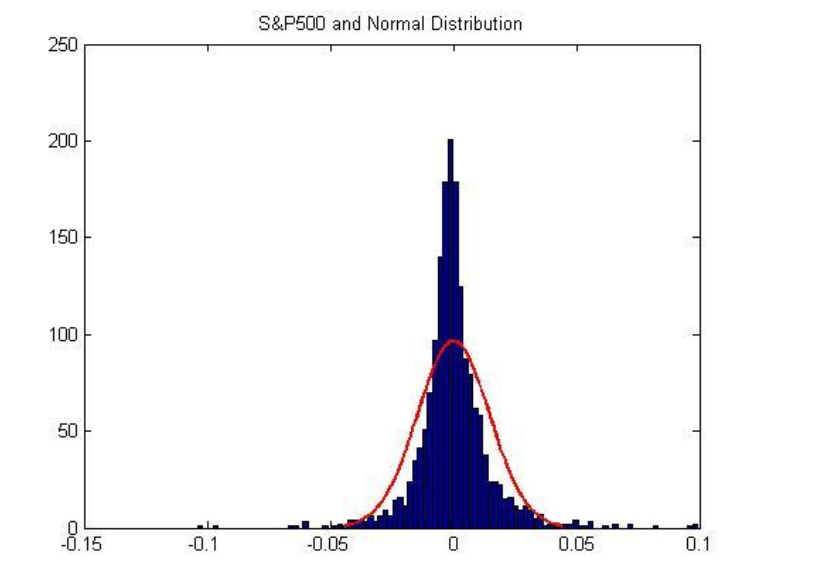
\includegraphics[width=0.6\textwidth]{sp500.png}
\end{figure}


Another imperfection of Black-Scholes model is the
volatility clustering: parameters of uncertainty change stochastically over time.

The best way to demonstrate the volatility clustering is plotting autocorrelations of
squared log-returns. This method helps see if the heteroscedasticity took place.
Heteroscedasticity is a violation of the constant error variance assumption. It occurs
if different observations’ errors have different variances. Obviously, in case of
financial market series we take volatility as the source of error.
The following figure shows high autocorrelations, i.e. our data is heteroscedastic, thus we have volatility clustering.\\
\begin{figure}[H]
    \centering
    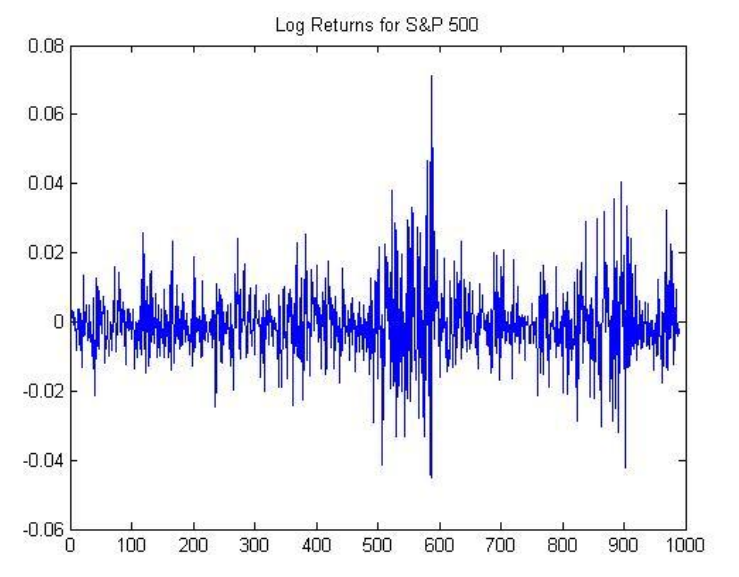
\includegraphics[width=0.6\textwidth]{log.png}
\end{figure}

So, GBM has no jumps in it and its volatility is constant, that is why such models like Heston or Merton are much more popular in practice (see section 1.2). Here we give some illustrations: \\

\begin{figure}[H]
    \centering
    \caption{GBM path in C++ with gnuplot}
    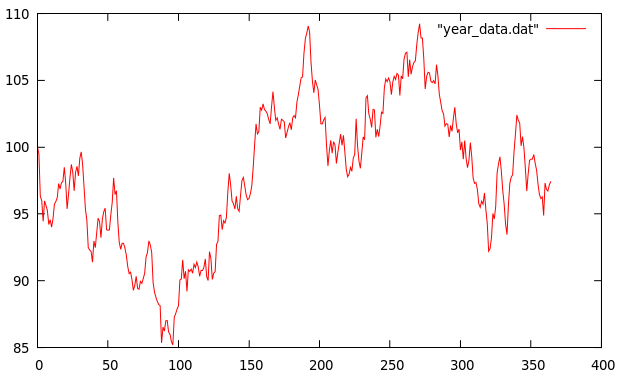
\includegraphics[width=0.8\textwidth]{gbmgnu.png}
    \caption{GBM path}
\end{figure}   





\begin{figure}[H]
    \centering
    \caption{Wiener and Wiener-Poisson process}
    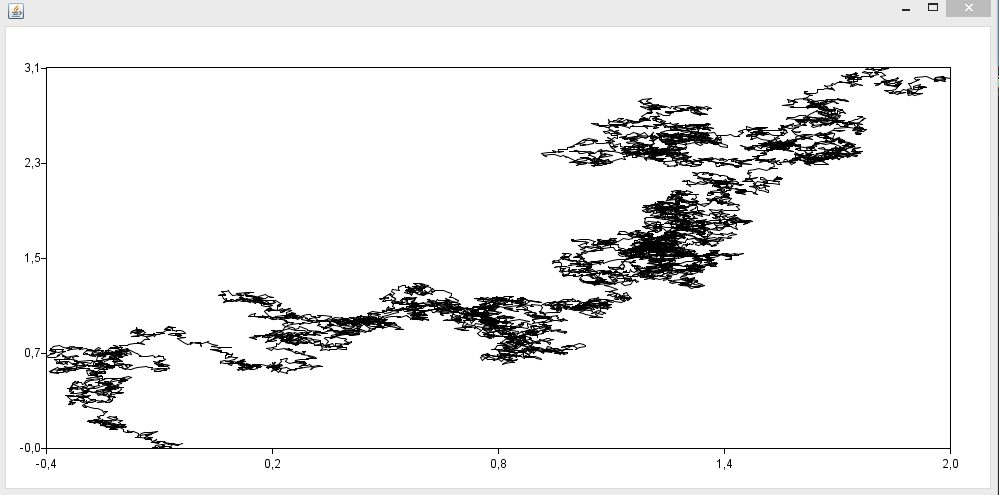
\includegraphics[width=0.55\textwidth]{brown.png}
\end{figure}

\begin{figure}[H]
    \centering
    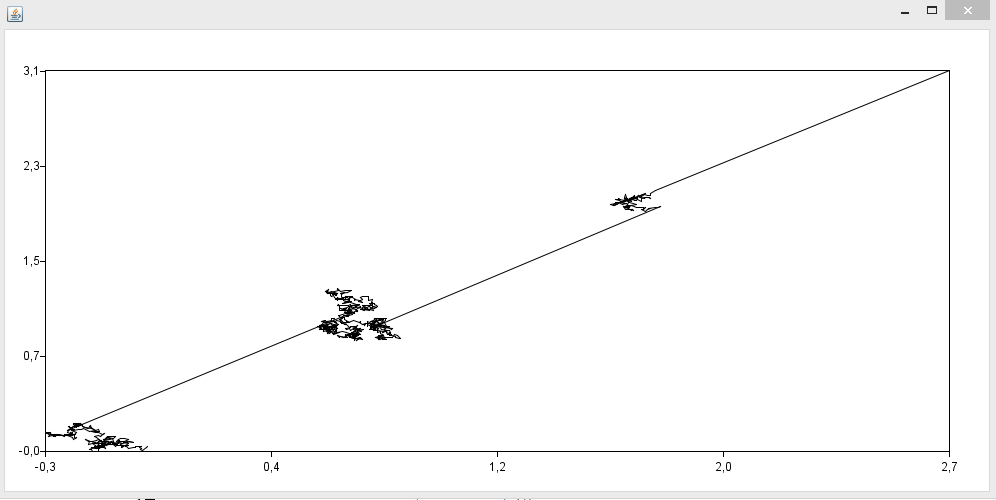
\includegraphics[width=0.55\textwidth]{poisson.png}
\end{figure}

\begin{figure}[H]
    \centering
    \caption{Black Scholes and Merton}
    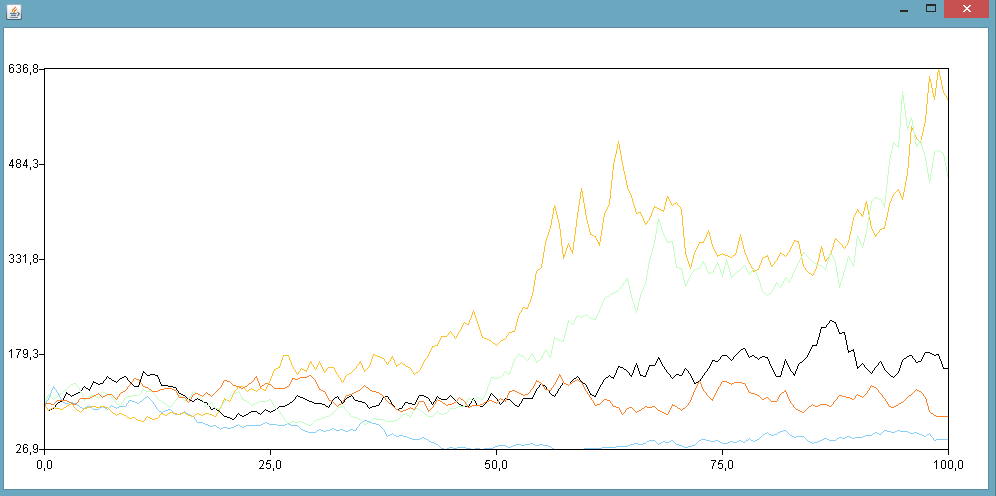
\includegraphics[width=0.55\textwidth]{wiener.png}
\end{figure}

\begin{figure}[H]
    \centering
    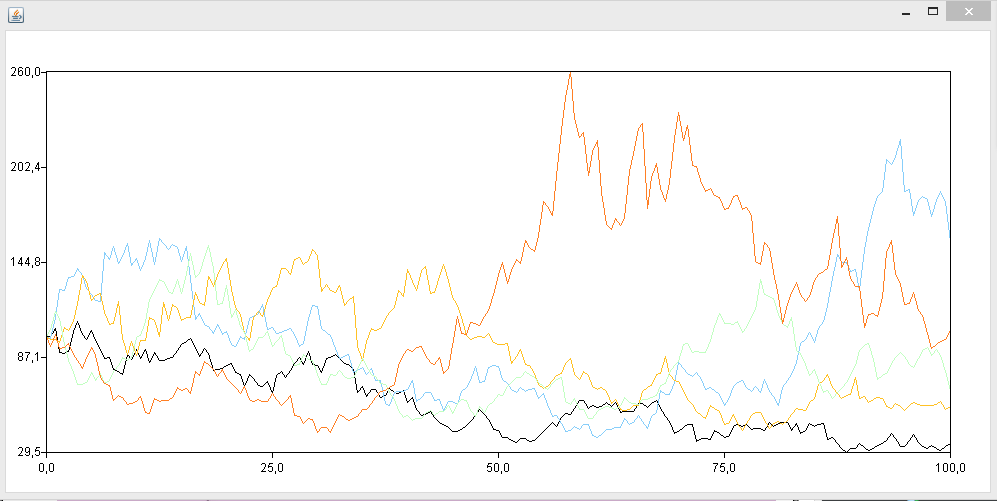
\includegraphics[width=0.55\textwidth]{merton.png}
\end{figure}



\section{ Black-Scholes pricing formulas }

Lets find the discounted expectation $e^{-rT}\mathbb{E}[max(S_T - K,0)]$ for a Vanilla Call option $C$. Please note, that we need to take in account that $\mu = r - d$ , where $d$ corresponds to a dividend yield. \\

$C = e ^{-rT} \mathbb{E} [max(S_0 e^{(r-d - \frac{\sigma^2}{2}) T + \sigma B_T} -K, 0)]$\\



$=\frac{1}{\sqrt{2 \pi} } \int_{\frac{\ln (\frac{K}{S_0}) - (r-d - \frac{\sigma^2}{2} )T}{\sigma \sqrt{T}}}^\infty (S_0 e^{\sigma \sqrt{T} x - (d+\frac{\sigma^2}{2} T)} - e^{-rT} K)e^{-\frac{x^2}{2}} dx $\\



$=e^{-dT} S_0 \frac{1}{\sqrt{2 \pi}} \int_{-d_2}^\infty e^{-\frac{(x- \sigma \sqrt{T})^2}{2}}dx - e^{-rT} K \frac{1}{\sqrt{2 \pi}} \int_{-d_2}^\infty e^{-\frac{x^2}{2}} dx $\\



$=e^{-dT} S_0 (1 - \mathcal{N}(-d_2-\sigma \sqrt{T}))-e^{-rT}K(1-\mathcal{N}(-d_2)) $\\


$=e^{-dT}S_0 \mathcal{N}(d_1)-e^{-rT}K\mathcal{N}(d_2))$\\
\newline
with
\begin{itemize}
\item
$ d_1 = \frac{\ln (\frac{S_0}{K}) + (r-d + \frac{\sigma^2}{2} )T}{\sigma \sqrt{T}} $ 
\item
$ d_2 = \frac{\ln (\frac{S_0}{K}) + (r-d - \frac{\sigma^2}{2} )T}{\sigma \sqrt{T}}  = d_1 -{\sigma \sqrt{T}}$ 

\end{itemize}
With similar computation we get a formula for Put option:\\

$P = e^{-rT}K\mathcal{N}(-d_2))-e^{-dT}S_0 \mathcal{N}(-d_1)$\\




















\chapter{Applying FEM}
\section{Derivation of Black-Scholes PDE}
\subsection{Economic insight}
Black-Scholes equation is a linear parabolic PDE with non-constant coefficients and non-homogeneous
boundary conditions and, possibly, non-differentiable or discontinuous final
conditions. Here we give its derivation:\\
We take the expression of a Geometric Brownian motion with $a(S,t)$ and $b(S,t)$ as coefficients:
\begin{equation}
dS = a(S,t)dt+b(S,t)dB
\end{equation}
Then we take a function $V \in C^2$ and with Ito's lemma we get :
\begin{equation}
dV(S,t) = \frac{\partial V}{\partial t}  + a(S,t) \frac{\partial V}{\partial S}  +    \frac{b(S,t)^2}{2}  \frac{\partial^2 V}{\partial S^2}) dt + b(S,t) \frac{\partial V}{\partial S}dB
\end{equation}
As the asset price follows GBM, let's do following changes: 
\begin{itemize}
\item $a(S,t)=S\mu$
\item $b(S,t)=S\sigma$
\end{itemize}
That give us:
\begin{equation}
dV(S(t),t) = (\frac{\partial V}{\partial t}  + S\mu \frac{\partial V}{\partial S}  +    \frac{\sigma^2 S^2}{2}  \frac{\partial^2 V}{\partial S^2}) dt + S\sigma \frac{\partial V}{\partial S}dB
\end{equation}
Now we consider a portfolio  with an option $V$ and "short" on some asset value $\Delta S$ - in other words, we use so called, \textit{delta-hedge portfolio} - the portfolio which value remains unchanged when small changes occur in the value of the underlying asset.\\
\begin{equation}
\Pi=V-\Delta S
\end{equation}
or with time inserted:
\begin{equation}
d\Pi=dV-\Delta dS
\end{equation}
Let's insert the last PDE and the GBM in our portfolio: 
\begin{equation}
d\Pi = ((\frac{\partial V}{\partial t}  + S\mu \frac{\partial V}{\partial S}  +    \frac{\sigma^2 S^2}{2}  \frac{\partial^2 V}{\partial S^2}) dt + S\sigma \frac{\partial V}{\partial S}dB-\Delta(S\mu dt+S\sigma dB)
\end{equation}
Now, in order to remove the random term $dB$, we fix $\Delta=\frac{\partial V}{\partial S}$:

\begin{equation}
d\Pi = (\frac{\partial V}{\partial t}  + S\mu \frac{\partial V}{\partial S}  +    \frac{\sigma^2 S^2}{2}  \frac{\partial^2 V}{\partial S^2} - S\mu  \frac{\partial V}{\partial S}) dt = (\frac{\partial V}{\partial t}+\frac{1}{2}\sigma^2 S^2\frac{\partial^2 V}{\partial S^2})dt
\end{equation}
Another purely financial concept, not discussed here, is \textit{arbitrage free market}, that is expressed as: 
\begin{equation}
d\Pi=r\Pi dt
\end{equation}
This concept is one of assumptions given in 3.1.\\
So , when substituting the portfolio and $d\Pi$ in the no-arbitrage expression, we get:
\begin{equation}
(\frac{\partial V}{\partial t}+\frac{1}{2}\sigma^2 S^2\frac{\partial^2 V}{\partial S^2})dt = r(V-\frac{\partial V}{\partial S}S)dt
\end{equation}
The final PDE comes out after we d1vide both sides by $dt$:
\begin{equation}
\frac{\partial V}{\partial t}+\frac{1}{2} \sigma^2 S^2\frac{\partial^2 V}{\partial S^2} + rS\frac{\partial V}{\partial S} - rV=0
\end{equation}

\subsection{PDE insight: Heat equation}

Here we give another derivation of Black-Scholes PDE : we'll transform it into a heat equation.\\
\begin{itemize}
\item $x=\ln \frac{S}{K} \Rightarrow S=Ke^x$
\item $\tau = \frac{\sigma^2}{2}(T-t) \Rightarrow t=T-\frac{2\tau}{\sigma^2}$
\item $U(x,\tau)=\frac{1}{K} V(S,t)=\frac{1}{K} V(Ke^x, T-2\frac{\tau}{\sigma^2}$
\end{itemize}
We apply the chain rule to partial derivatives:
\begin{itemize}
\item $\frac{\partial V}{\partial t}=K \frac{\partial U}{\partial \tau}\frac{\partial \tau}{\partial t} =\frac{-K\sigma^2}{2} \frac{\partial U}{\partial \tau} $
\item $\frac{\partial V}{\partial S}=K \frac{\partial U}{\partial x}\frac{\partial x}{\partial S} =\frac{K}{S} \frac{\partial U}{\partial x}=e^{-x} \frac{\partial U}{\partial x} $
\item  $\frac{\partial^2 V}{\partial S^2} = \frac{e^{-2x}}{K}(\frac{\partial^2 U}{\partial x^2}-\frac{\partial U}{\partial x})$
\end{itemize}
Recall the initial PDE:
\begin{equation}
\frac{\partial C}{\partial t}+\frac{1}{2} \sigma^2 S^2\frac{\partial^2 C}{\partial S(t)^2} + rS(t)\frac{\partial C}{\partial S(t)} - rC=0
\end{equation}
Then, we substitute the new terms in it:
\begin{equation}
\frac{-K\sigma^2}{2} \frac{\partial U}{\partial \tau}+rKe^xe^{-x} \frac{\partial U}{\partial x}+\frac{1}{2}\sigma^2K^2\frac{e^{-2x}}{K}(\frac{\partial^2 U}{\partial x^2}-\frac{\partial U}{\partial x})-rU=0
\end{equation}
which simplifies to
\begin{equation}
-\frac{\partial U}{\partial \tau} + (k-1)\frac{\partial U}{\partial x}+\frac{\partial^2 U}{\partial x^2}-kU=0
\end{equation}
with $k=\frac{2r}{\sigma^2}$.\\
Now, we update the boundary conditions w.r.t. the initial transforms:
$U_0(x_T)=U(x_T,0)=\frac{1}{K}V(S_T-K)^+=\frac{1}{K}(Ke^{x_T}-K)^+=(e^{x_T}-1)^+$\\
Lets do one more transform:
$W(x,\tau) = e^{\alpha x+\beta^2 \tau}U(x,\tau)$ with:
\begin{itemize}
\item $\alpha = \frac{1}{2}(k-1)$
\item $\beta = \frac{1}{2}(k+1)=\alpha+1$
\end{itemize}
This will convert our equation in a Heat equation. So, the partial derivatives of $U$ it terms of $W$ are given bellow:
\begin{itemize}
\item $\frac{\partial U}{\partial \tau} = e^{-\alpha x-\beta^2\tau}(\frac{\partial W}{\partial \tau} - W(x,\tau)\beta^2)$ 
\item $\frac{\partial U}{\partial x} = e^{-\alpha x-\beta^2\tau}(\frac{\partial W}{\partial x} - \alpha W(x,\tau))$
\item $\frac{\partial^2 U}{\partial x^2} = e^{-\alpha x-\beta^2\tau}(\alpha^2 W(x,\tau) - 2\alpha\frac{\partial W}{\partial x} + \frac{\partial^2 W}{\partial x^2}$
\end{itemize}

Next, we insert these derivatives in our equation: 
\begin{equation}
\beta^2W(x,\tau) - \frac{\partial W}{\partial \tau} + (k-1)[\alpha W(x,\tau)+\frac{\partial W}{\partial x}]+\alpha W(x,\tau)-2\alpha\frac{\partial W}{\partial x} + \frac{\partial^2 W}{\partial x^2}-k W(x,\tau)=0
\end{equation}
After all simplifications we finally get:
\begin{equation}
\frac{\partial W}{\partial \tau} = \frac{\partial^2 W}{\partial x^2}
\end{equation}
We also update the boundary conditions:
$W_0(x_T) = W(x_T,0)=e^{\alpha x_T}U(x_T,0)=(e^{(\alpha+1)x_T}-e^{\alpha x_T})^+ = (e^{\beta x_T} - e^{\alpha x_T})^+.$\\

The transformation from $V$ to $W$ is therefore:
\begin{equation}
V(S,t) = \frac{1}{K}e^{-\alpha x-\beta^2\tau}W(x,\tau)
\end{equation}
\newline
\textbf{Obtain a Call price}:
Since $W(x,\tau)$ follows the heat equation, it has "the same" solution, which we know.
\begin{equation}
W(x,\tau) = \frac{1}{\sqrt{4\pi \tau}} \int_{-\infty}^\infty e^{-(x-\xi)^2/4\tau}W_0(\xi)d\xi= 
\frac{1}{\sqrt{4\pi \tau}} \int_{-\infty}^\infty e^{-(x-\xi)^2/4\tau}(e^{\beta \xi}-e^{\alpha \xi})^+d\xi
\end{equation}
We make the following change of variables: $z=\frac{\xi - x}{\sqrt{2\tau}} \Rightarrow \xi = \sqrt{2\tau}z$ and $d\xi=\sqrt{2\tau}dz $. As result:
\begin{equation}
W(x,\tau) = \frac{1}{\sqrt{2\pi}} \int_{-\infty}^\infty exp(-\frac{1}{2}z^2) \times exp ( \beta [\sqrt{2\tau}z+x]-\alpha[\sqrt{2\tau}z+x])^+dz
\end{equation}
Now, lets break up the integral (Note, that the integral is non zero only if $\beta[\sqrt{2\tau}z+x]>\alpha[\sqrt{2\tau}z+x]$, in other words $z>-\frac{x}{\sqrt{2\tau}}$):\\
\begin{equation}
W(x, \tau)=\frac{1}{\sqrt{2\pi}} \int_{-x/\sqrt{2\tau}}^\infty exp(-\frac{1}{2}z^2)exp (\beta [\sqrt{2\tau}z+x])dz - \frac{1}{\sqrt{2\pi}} \int_{-x/\sqrt{2\tau}}^\infty exp(-\frac{1}{2}z^2)exp (\alpha[\sqrt{2\tau}z+x])dz = I_1-I_2
\end{equation}

We complete the square in $I_1$:
$-\frac{1}{2}z^2+\beta\sqrt{2\tau}z+\beta x = -\frac{1}{2(z-\beta}\sqrt{2\tau})^2+\beta+\beta^2\tau$ \\
$ y = z- \beta \sqrt{2\tau} 
\Rightarrow
I_1 = e^{\beta x + \beta^2\tau}\frac{1}{\sqrt{2\pi}} \int_{-x/\sqrt{2\tau}}^\infty e^{  -\frac{1}{2} (z-\beta\sqrt{2\tau})^2} dz$   \\ 
After simplifications, the integrals become:
$I_1 = e^{\beta x + \beta^2\tau}\mathcal{N} (\frac{x}{\sqrt{2\tau}} + \beta \sqrt{2\tau})$\\
$I_2 = e^{\alpha x + \alpha^2\tau}\mathcal{N} (\frac{x}{\sqrt{2\tau}} + \alpha \sqrt{2\tau})$
We inverse the initial transformation and we get 
\begin{itemize}
\item $\frac{x}{\sqrt{2\tau}}+\beta\sqrt{2\tau}=\frac{\ln \frac{S}{K}+(r+\frac{\sigma^2}{2})(T-t)}{\sigma\sqrt{T-t}}=d_1 $
\item $\frac{x}{\sqrt{2\tau}} + \alpha\sqrt{2\tau}=d_1-\sigma\sqrt{T-t} = d_2 $
\end{itemize}
$I_1 = exp(\beta x + \beta^2 \tau) \mathcal{N}(d_1)$\\
$I_2 = exp(\alpha x + \alpha^2 \tau) \mathcal{N}(d_2)$\\
The solution is there for:
\begin{equation}
W(x,\tau) = I_1-I_2=exp(\beta x + \beta^2 \tau) \mathcal{N}(d_1)-exp(\alpha x + \alpha^2 \tau) \mathcal{N}(d_2)
\end{equation}
Using the last equation and the transformation form $V$ to $W$ we got before, we obtain:
\begin{equation}
V(S,t) = Ke^{-\alpha x -\beta ^2 \tau}W(x,\tau) = 
Ke^{-\alpha x -\beta ^2 \tau}(I_1-I_2)
\end{equation}
So, after all the substitutions we get:\\

$Ke^{-\alpha x -\beta ^2 \tau}exp(\beta x + \beta^2 \tau) \mathcal{N}(d_1)+Ke^{-\alpha x -\beta ^2 \tau}exp(\alpha x + \alpha^2 \tau) \mathcal{N}(d_2)=Ke^{(\beta-\alpha)x}\mathcal{N}(d_1) + Ke^{(\alpha^2-\beta^2)\tau}\mathcal{N}(d_2)=$

\begin{equation}
=S\mathcal{N}(d_1) - Ke^{-r(T-t)}\mathcal{N}(d_2)
\end{equation}


Since $\alpha^2-\beta^2 = -\frac{2r}{\sigma^2}$.



















\section{Boundary conditions}
\begin{itemize}


\item Call Option\\
When fixing final, initial and boundary conditions we use economical arguments. Final condition is known and well posed : at time $T$ worth $0$ or $S-K$. If $S=0$ then $C=0$. If $S\longrightarrow\infty$, the option value is the asset price corrected  by the dividend minus the exercise price corrected by the case if the holder had invested his money on the bank, so $C(S,t) = e^{-dT}S_0-e^{-rT}K$. So our final problem is:
\begin{equation}
\frac{\partial C}{\partial t}+\frac{1}{2} \sigma^2 S^2\frac{\partial^2 C}{\partial S^2} + rS\frac{\partial C}{\partial S} - rC=0
\end{equation}
\begin{alignat*}{2}
C(0,t)=0\\
C(S,t) = e^{-dT}S_0-e^{-rT}K$  when $S\longrightarrow \infty \\
C(S,T) = max(S-E,0)
\end{alignat*}

\item Put Option\\
The same logic gives us conditions for put option.
\begin{equation}
\frac{\partial P}{\partial t}-\frac{1}{2} \sigma^2 S^2\frac{\partial^2 P}{\partial S^2} - rS\frac{\partial P}{\partial S} + rP=0
\end{equation}
\begin{alignat*}{2}
P(0,t) =e^{-rT}K\\
P(S,t) = 0$  when $S\longrightarrow \infty \\
P(S,T) = max(E-S,0)
\end{alignat*}
\end{itemize}
\section{Weak Formulation}

Consider a vanilla put option with maturity $T$ and payoff function $u_0 $. Let $u$ be the pricing function, i.e., the price of the option at time $T − t$ and when the spot price is $S$ is $u(S, t)$. The function $u$ solves the initial SDE:
\begin{equation}
\frac{\partial u}{\partial t}-\frac{1}{2} \sigma^2 S^2\frac{\partial^2 u}{\partial S^2} - rS\frac{\partial u }{\partial S} + ru=0
\end{equation}

Now lets multiply it by a test function, that lives in Weighted Sobolev space : $ \forall u \in V,  V=\{ v \in L^2(\mathbb{R}_+) : S\frac{\partial v}{\partial S} \in L^2(\mathbb{R}_+) \}$ and integrate the whole expression. As always , we apply the integration by parts and obtain:
\begin{equation}
\frac{d}{dt} (\int_{\mathbb{R}^+} u(S,t) w(S)dS) + a_t(v, w) = 0,
\end{equation}
where $a_t$ is a bilinear form defined as:
\begin{equation}
a_t(v,w) = \int_{\mathbb{R}^+} (\frac{1}{2} S^2\sigma^2(S,t)\frac{\partial v}{\partial S}\frac{\partial w}{\partial S} + r(t)vw)ds + 
\int_{\mathbb{R}^+} (-r(t)+\sigma^2(S,t) + S\sigma(S,t)\frac{\partial \sigma}{\partial S}(S,t))S\frac{\partial v}{\partial S}wdS.
\end{equation}



\section{Existence and Uniqueness}
Note that the first proof uses economic insight, so can not be seen as fully accurate proof. While the second one is rarely given in books in computational finance as it demands deep knowledge in stochastic calculus.  
\subsection{Economic insight}

\begin{itemize}
\item As the volatility is always positive and bounded, we can conclude that $a_t$ is continuous on $V$, càd there exists a positive constant $M$, such that for all $v,w \in V$,
\begin{equation}
|a_t(v,w)| \leq M|v|_V |w|_V.
\end{equation} 
\item The bilinear form is also \textbf{Gârding} coercive, càd:
\begin{equation}
a_t(v,v) \geq C_1 ||v||_V^2 - C_2 ||v||_{L^2}^2.
\end{equation}
\end{itemize}
So, under these conditions we may say that by Lax-Milgram if $u_0 \in L^2$ then it is the unique  solution and we can write the weak formulation:
\\
\begin{alignat*}{2}
$Find  $u \in \mathcal{C}^0([0;T]), u \in L^2 \cap V\\
\forall v\in V, (\frac{\partial u}{\partial t}(t), v) + a_t(u(t), v)=0.\\
u(0,t)=0\\
u(S,t) = e^{-dT}S_0-e^{-rT}K$  when $S\longrightarrow \infty \\
u(S,T) = max(S-E,0)
\end{alignat*}


\subsection{PDE insight}
\textbf{Gronwall inequality}\\
Let $v(t)$ be a non-negative function such that 
\begin{equation}
v(t) \leqC+A\int_0^t v(s) ds
\end{equation}
for some constants C,A. Then 
\begin{equation}
v(t) \leq C exp (At)
\end{equation}
for all $0 \leq t \leq T$.\\
\newline



\textbf{Theorem} of existence and uniqueness of the solution for a SDE:\\
Let $T>0$. Let $b(.,.):[0,T] \times \mathbb{R}^n \longrightarrow \mathbb{R}^n$ and  $ \sigma(.,.):[0,T] \times \mathbb{R}^n \longrightarrow \mathbb{R}^{n \times m}$ be measurable functions, satisfying two following properties:
\begin{equation}
|b(t,x)|+|\sigma(t,x)| \leq C(1+|x|),  
\end{equation}
with  $ x\in \mathbb{R}, t\in [0,T],$ for some constant $C$, (where $|\sigma |^2=\sum|\sigma_{ij}|^2)$ and (Lipschitz property):

\begin{equation}
|b(t,x)-b(t,y)|+|\sigma(t,x)-\sigma(t,y)| \leq D |x-y|,  
\end{equation}
with  $ x, y \in \mathbb{R}, t\in [0,T],$ for some constant $D$.\\
Let Z be a random variable which is independent of the $\sigma$ -algebra $\mathbb{F}_\infty^{(m)}$ generated by $B_s(.)$, $s>0$,  such that  $\mathbb{E}[|Z|^2]<\infty$.\\
Then the stochastic SDE $dX_t = b(t,X_t)dt + \sigma(t, X_t)dB_t $  with $X_0=Z$ has a unique solution $X_t(w)$ with the property that $X_t(w)$ is adapted to the filtration $\mathbb{F}_t^Z$ and $B_s(.)$, $s<t$
 and $\mathbb{E}[\int_0^T |X_t|^2dt]<\infty$

\textbf{Proof:}\\
The uniqueness follows from Itô's isometry and Lipschitz property.\\
Let $X_1(t,w)=X_t(w)$ and $X_2(t,w)=X_t'(w)$ be solutions with initial values $Z,Z'$, i.e. $X_1(0,w)=Z(w), X_2(0,w)=Z'(w), w\in \Omega$.\\
We put $a(s,w) = b(s,X_s)-b(s,X_s')$ and $\gamma = \sigma(s,X_s)-\sigma(s,X_s')$. Then,\\
$\mathbb{E} [|X_t-X_t'|^2] = \mathbb{E} [(Z-Z' + \int_0^t ads + \int_0^t \gamma dB_s)^2]$\\
$\leq 3\mathbb{E} [|Z-Z'|^2] + 3\mathbb{E}[(\int_0^t ads)^2] + 3 \mathbb{E}[(\int_0^t \gamma dB_s)^2]$\\
$\leq 3\mathbb{E} [|Z-Z'|^2] +3t\mathbb{E} [\int_0^t a^2 ds] + 3\mathbb{E}[\int_0^t \gamma^2 ds)^2]$\\
$\leq 3\mathbb{E} [|Z-Z'|^2] +3(t+1)D^2 \int_0^t \mathbb{E} [|X_s-X_s'|^2]ds$\\
\newline
So the function $v(t) = \mathbb{E}[|X_t-X_t'|^2]$ with $0\leq t\leq T$ satisfies
\begin{equation}
v(t) \leq F+A\int_0^t v(s) ds
\end{equation}
where $F=3\mathbb{E} [|Z-Z'|^2]$ and $A=3(1+T)D^2$.\\
By Gronwall inequity we conclude:
\begin{equation}
v(t) \leq F e^{At}
\end{equation}
Lets now assume that $Z=Z'$, then $F=0$ and so $v(t)=0$, hence
\begin{equation}
P[|X_t-X_t'|]=0
\end{equation}
By continuity of $t\longrightarrow|X_t-X_t'|$ it follows that 
\begin{equation}
P[|X_1(t,w) - X_2(t,w)|]=0
\end{equation}
Thus, the solution is unique.\\
Now, lets prove the existence.\\
Define $Y_t^{0}=X_0$ and $Y_t^{k}=Y_t^{k}(w)$, so we get:
\begin{equation}
Y_t^{k+1} = X_0+\int_0^t b(s,Y_s^{k})ds + \int_0^t \sigma(s,Y_s^{(k)})dB_s
\end{equation}
Then, with similar computation as for uniqueness we get:
\begin{equation}
\mathbb{E}[|Y_t^{k+1}-Y_t^{(k)}|^2]\leq (1+T)3D^2\int_0^t \mathbb{E}[|Y_s^{(k)} - Y_s^{(k-1)}|^2]ds
\end{equation}
and
\begin{equation}
\mathbb{E}[(Y_t^{(1)}-Y_t^{(0)}|^2] \leq 2C^2t^2(1+\mathbb{E}[|X_0|^2])+2C^2t(1+\mathbb{E}[|X_0|^2]) \leq A_1 t
\end{equation}
where $A_1$ is a constant that depends on $C,T$ and $\mathbb{E}[|X_0|^2]$. So by induction on $k$ we obtain:
\begin{equation}
\mathbb{E} [|Y_t^{k+1)}-Y_t^{(k)}|^2] \leq \frac{A_2^{k+1}t^{k+1}}{(k+1)!}
\end{equation}
where $A_2$ is a suitable constant depending on $C,D,T$ and $\mathbb{E}[|X_0|^2]$.

Hence, if $\lambda$ denotes Lebesgue measure on $[0,T]$ with $m>n>0$ we get:\\
$||Y_t^{(m)}- Y_t^{(n)}||_{L^2(\lambda \times P)} = ||\sum_{k=n}^{m-1} Y_t^{(k+1)} -Y_t^{(k)} ||_{L^2(\lambda \times P)}$\\
$= \sum_{k=n}^{m-1} (\mathbb{E}[\int_0^T |Y_t^{(k+1)} - Y_t^{(k)} |^2 dt])^{1/2}$\\
$ \leq \sum_{k=n}^{m-1} ( \int_0^T   \frac{A_2^{k+1}t^{k+1}}{(k+1)!} dt)^{1/2} = \sum_{k=n}^{m-1} (  \frac{A_2^{k+1}T^{k+2}}{(k+2)!} dt)^{1/2} \longrightarrow 0$\\
as $m,n \longrightarrow\infty$.\\
\newline
Therefore $ \{Y_t^{(n)} \}^\infty_{n=0}$ is a Cauchy sequence in $L^2(\lambda \times P) \Rightarrow  \{Y_t^{(n)} \}^\infty_{n=0}$ converges. Lets define its limit by $X_t$.\\
Then $X_t$ is $\mathcal{F}_t^Z$-measurable for all $t$.\\
Our last step is to prove that $X_t$ follows the given PDE.\\
Fot all $n,t$ we have 
\begin{equation}
Y_t^{(n+1)} =X_0+\int_0^t b(s,Y_s^{(n)})ds+\int_0^t \sigma (s,Y_s^{(n)})dB_s
\end{equation}
When $n\longrightarrow \infty$, then by Hölder inequity we obtain:
\begin{equation}
\int_0^t b(s,Y_s^{(n)})ds \longrightarrow \int_0^t b(s,X_s)ds
\end{equation}
And by Itö ismometry the third terms becomes
\begin{equation}
\int_0^t \sigma(s,Y_s^{(n)})dB_s \longrightarrow \int_0^t \sigma (s,X_s)dB_s
\end{equation}
So we conclude that for $\all t \in [0,T]$ we have
\begin{equation}
X_t=X_0 + \int_0^t b(s,X_s)ds + \int_0^t \sigma (s, X_s)dB_s
\end{equation}
\square
\section{Mesh Adaptation and Delaunay triangulation}
Mesh adaptation is an important tool in problems with free boundary. The procedure is done w.r.t. Delanay algorithm and keeps the error of interpolation bounded by:
\begin{equation}
||u-u_h||<C|| \nabla ( \nabla u)h^2
\end{equation}
where $\nabla (\nabla u)$ is a Hessian matrix of u.\\
The, so called, Delaunay triangulation helps to create a "good" mesh : no obtuse triangles, neighbour triangles have more or less the same size.\\
In other words, the Delaunay triangulation create a mesh where for each edge the circle circumscribing one triangle does not contain the fourth vertex.

\begin{figure}[H]
    \centering
    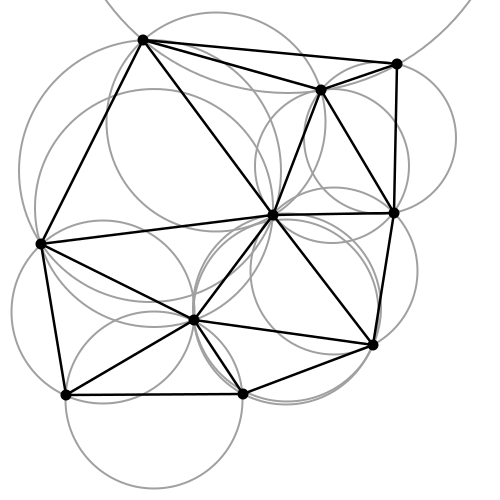
\includegraphics[width=0.4\textwidth]{Delaunay.png}
    \caption{ Delaunay triangulation}
\end{figure}

In freefem++ the mesh adaptation is easily done with \textbf{adaptmesh} command. 




\section{Numerical results}
We use the implicit scheme.
\subsection{FreeFem++}
\textbf{BlackScholes 1D}
\begin{itemize}
\item {Vanilla put, $K=100$}\\
With higher $\sigma$ the breakeven point is less obvious.
\begin{figure}[H]
   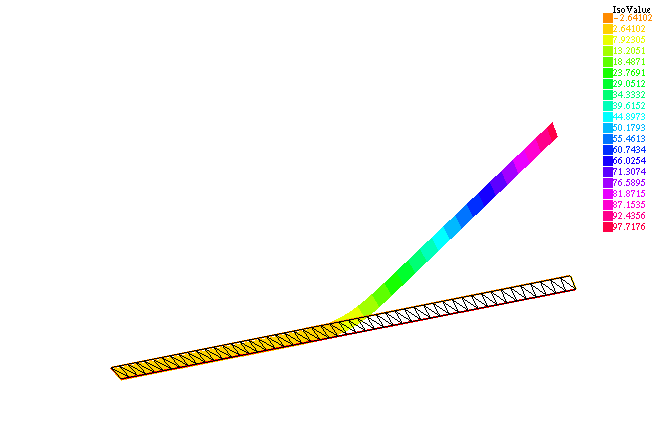
\includegraphics[width=0.475\textwidth]{s01.png}
   \hfill
   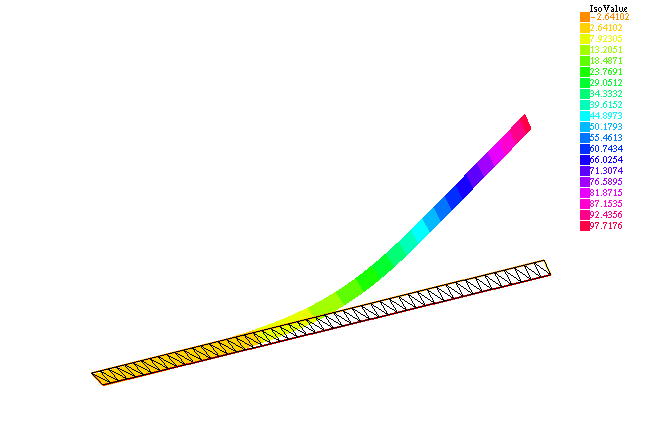
\includegraphics[width=0.475\textwidth]{s03.png}
    \caption{ $\sigma=0.1$ and $\sigma=0.3$}
\end{figure}
\item {Delta for Vanilla put, $K=100$}\\
With higher $\sigma$  option price changes slowly w.r.t. asset price. 
\begin{figure}[H]
   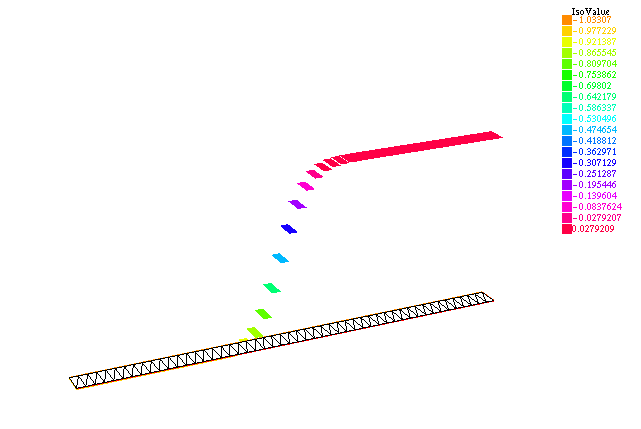
\includegraphics[width=0.475\textwidth]{d01.png}
   \hfill
   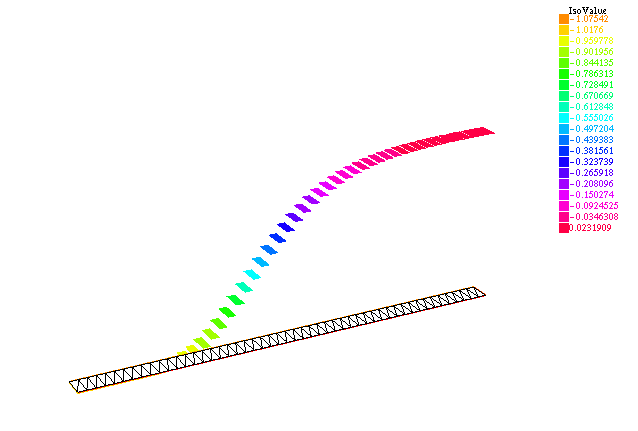
\includegraphics[width=0.475\textwidth]{d03.png}
    \caption{ Delta for $\sigma=0.1$ and $\sigma=0.3$}
\end{figure}
Same output line until the barrier is reached when the line drops. If barrier is $\geq K$, then no payoff.
\item {Barrier put, $K=100$}
\begin{figure}[H]
   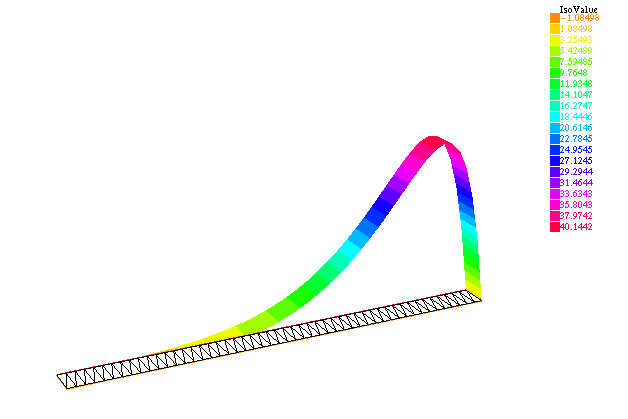
\includegraphics[width=0.300\textwidth]{b30.png}
   \hfill
   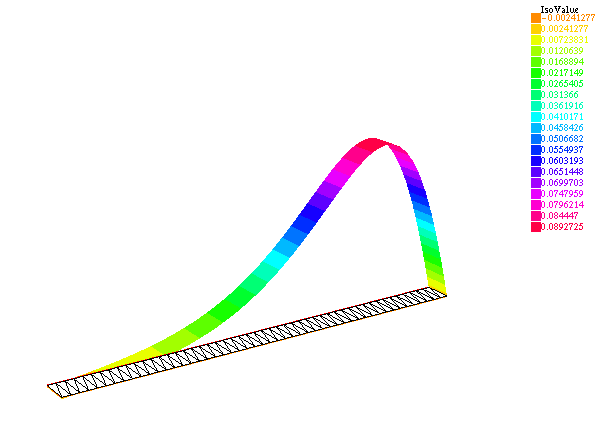
\includegraphics[width=0.300\textwidth]{b90.png}
	\hfill   
   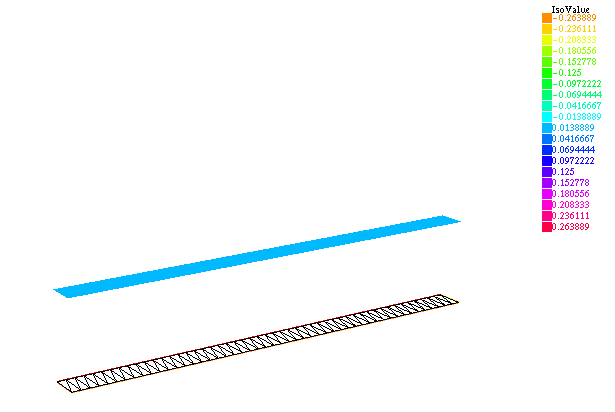
\includegraphics[width=0.300\textwidth]{b100.png}
    \caption{ barriers = $30,90,100$}
\end{figure}


\end{itemize}


\textbf{Black-Scholes 2D}
\begin{itemize}
\item {Classic asymmetric data}



\begin{figure}[H]
   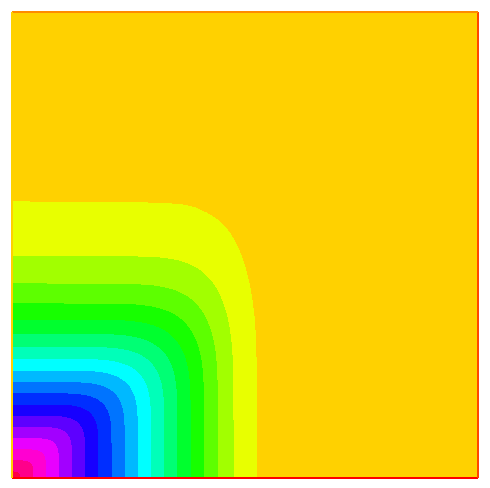
\includegraphics[width=0.475\textwidth]{bs1a.png}
   \hfill
   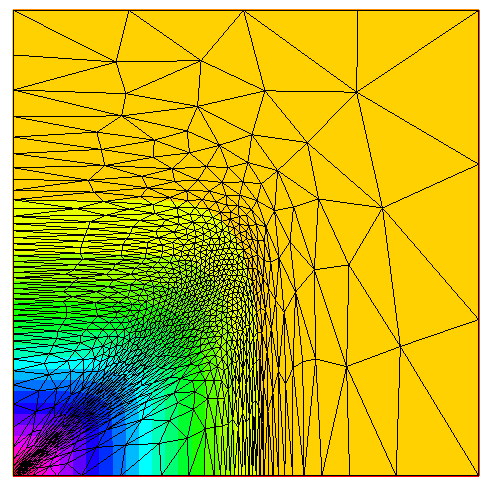
\includegraphics[width=0.475\textwidth]{bs1b.png}
   \caption{PDE : $\sigma_x=0.1, \sigma_y=0.3, \rho=0.3$}
\end{figure}


\item {Low volatility with high correlation}
\begin{figure}[H]
   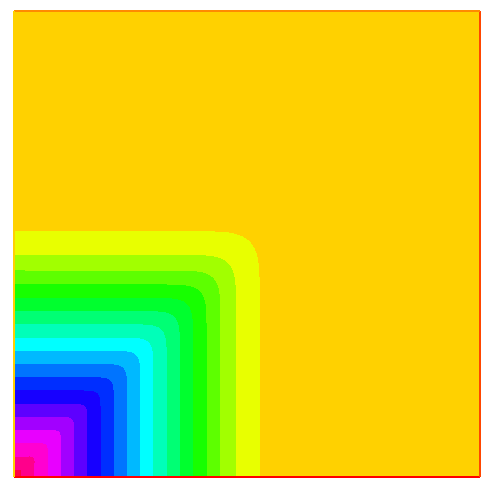
\includegraphics[width=0.475\textwidth]{bs2a.png}
   \hfill
   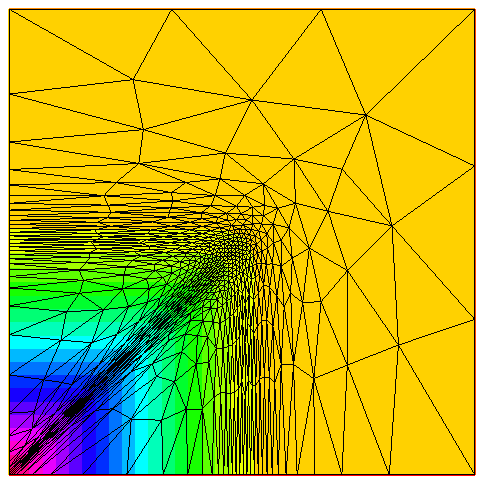
\includegraphics[width=0.475\textwidth]{bs2b.png}
    \caption{ PDE : $\sigma_x=0.1, \sigma_y=0.1, \rho=0.6$}
\end{figure}




\item {High volatility but low correlation}
\begin{figure}[H]
   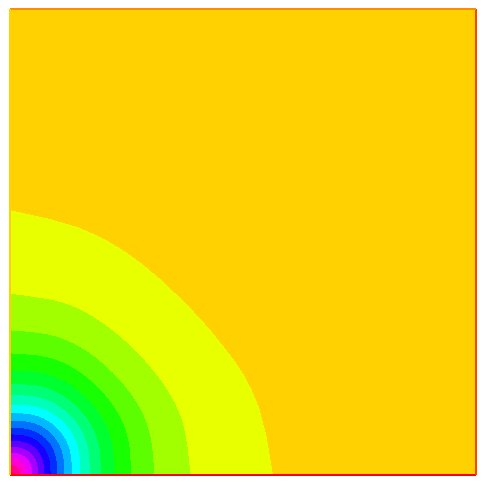
\includegraphics[width=0.475\textwidth]{bs3a.png}
   \hfill
   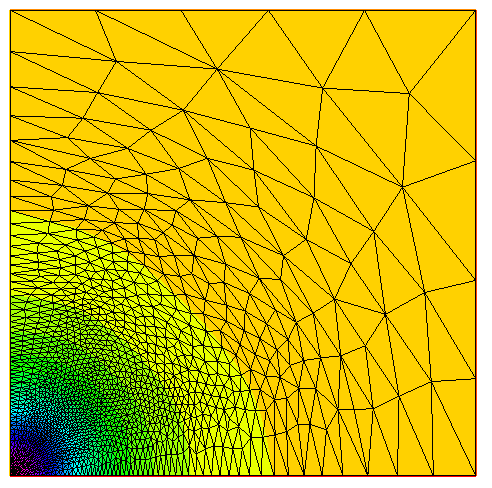
\includegraphics[width=0.475\textwidth]{bs3b.png}
    \caption{ PDE : $\sigma_x=0.6, \sigma_y=0.6, \rho=0.3$}
\end{figure}





\item {High volatility with high correlation}
\begin{figure}[H]
   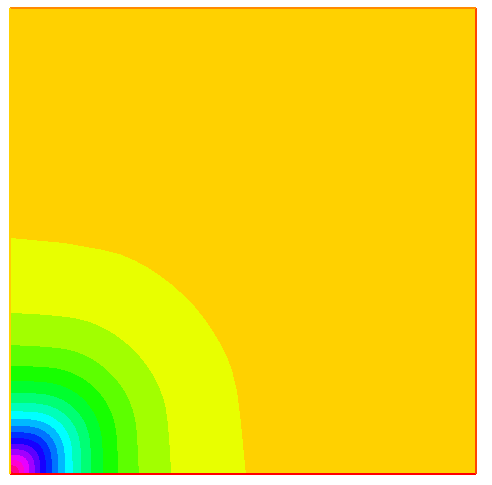
\includegraphics[width=0.475\textwidth]{bs4a.png}
   \hfill
   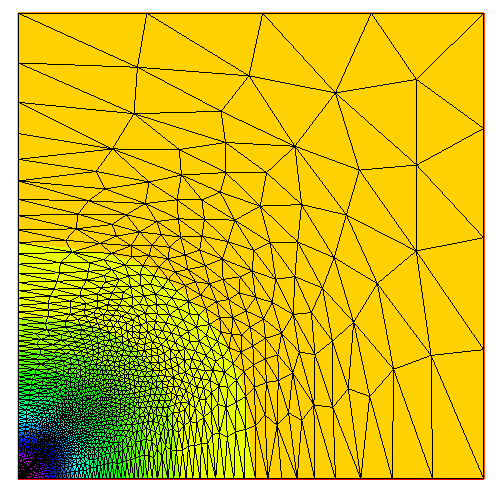
\includegraphics[width=0.475\textwidth]{bs4b.png}
    \caption{ PDE :$\sigma_x=0.6, \sigma_y=0.6, \rho=0.6$}
\end{figure}




\subsection{Fell++}
No export produced.
\begin{lstlisting}[backgroundcolor = \color{light-gray}]
 #include <feel/feel.hpp>

using namespace Feel;
inline
po::options_description
makeOptions()
{
po::options_description blackscholesoptions ("BS options");
blackscholesoptions.add_options()
        ("T", po::value<double>()->default_value(1.), "Time to maturity")
        ("K", po::value<double>()->default_value(1.), "Strike price")
        ("r", po::value<double>()->default_value(1.),"Interest rate")
        ("sigmax", po::value<double>()->default_value(1.),"sigma x")
        ("sigmay", po::value<double>()->default_value(1.),"sigma y")
        ("rho", po::value<double>()->default_value(1.),"rho")
        ("mu", po::value<double>()->default_value(1.),"mu")
        ("dt", po::value<double>()->default_value(1.),"dt")
        ;
        return  blackscholesoptions.add( backend_options("bs"));
}

int main (int argc, char* argv[])
{

        Environment env(_argc = argc, _argv=argv,
        _desc=makeOptions(),
        _about=about(_name="mymesh",
                     _author="Feel++ Consortium",
                     _email="feelpp-devel@feelpp.org"));

//loading a created mesh

        auto mesh = loadMesh(_mesh=new Mesh<Simplex<2>>,_filename = "square.geo");

//mesh adaptation - TODO

//determine space

        auto Xh = Pch<1>(mesh);


//initialisation of elements

        auto u=Xh->element("u");
        auto u1=Xh->element("u1");
        auto uold=Xh->element("uold");
auto v = Xh->element("v");

//initialisation of parameters

        double T=doption(_name="T"); //Time to maturiry
        double K=doption(_name="K"); //Strike price
        double r=doption(_name="r"); //Interest rate
        double sigmax=doption(_name="sigmax"); //Volatility for option A
        double sigmay=doption(_name="sigmay"); //Volatility for option B
        double rho = doption(_name="rho"); //Correlation between A and B
        double mu = doption(_name="mu"); //Drift rate
        double dt = doption(_name="dt"); //Time step
        u1.on(_range=elements(mesh), _expr=max(K-max(Px(),Py()),0.));
//additional functions

        auto xvel = -Px()*r + Px()*sigmax*sigmax+Px()*rho*sigmax*sigmay/2;
        auto yvel = -Py()*r + Py()*sigmay*sigmay+Py()*rho*sigmax*sigmay/2;

//initialisation of forms
        auto l = form1(_test=Xh);
        auto a = form2(_trial=Xh, _test=Xh);

//export
        auto e = exporter(_mesh = mesh);



//iteration

        for (double t=dt; t<T; t+=dt){
        u=u1;
        l.zero();
        uold = u;
        a=integrate(_range=elements(mesh),_expr =( (gradt(u)*vec(xvel,yvel))*id(v)));
        a+=integrate(_range=elements(mesh), _expr= ((idt(u)*id(v)*(r+(1/dt)))+dxt(u)*dx(v)*(sigmax*Px())*(sigmax*Px())/2+dyt(u)*dy(v)*(sigmay*Py())*(sigmay*Py())/2+(dyt(u)*dx(v) + dxt(uold)*dy(v))*rho*sigmax*sigmay*Px()*Py()/2) );

        a+=on(_range=markedfaces(mesh, "out"), _rhs=l, _element=u,_expr=cst(0.) );
        a+=on(_range=markedfaces(mesh,"in"), _rhs=l, _element=u,_expr=max(K-max(Px(),Py()),0.));
        a.solve(_solution=u, _rhs=l, _name="bs");
        Feel::cout<<"sol"<<u<<"\n";
//      e->step(t)->add("u",u);
//      e->save();
};
}
\end{lstlisting}


\chapter{Applying FDM}
\section{Overview}
Nowadays, most of financial researches use Finite Difference method to find the solution to stochastic PDE. The reason for it is that FDM is less labour and time consuming, and thus cheaper. This chapter explains the underlying idea of the method and shows its explicit implementation in C++.    \\
FDM is a discretization method used to solve parabolic PDE. There are three main schemes : 
\begin{itemize}
\item Forward-Time Central-Space (FTCS) or Explicit
\item Backward-Time Central-Space (BTCS)or Implicit
\item Central-Time Central-Space (CTCS) or Crank-Nickolson 
\end{itemize}
In numerical results we used Explicit method, so here we give it in detail.  \\
First, we find express small changes in $V(S,t)$ using Taylor's series:
\begin{itemize}[label=$\bullet$]
\item $V(S+\Delta S, t) = V(S,t)+\Delta S \frac{\partial V}{\partial S}+\frac{1}{2}(\Delta S)^2 \frac{\partial^2 V}{\partial S^2} + O((\Delta S)^3)  $
\item $V(S-\Delta S, t) = V(S,t)-\Delta S \frac{\partial V}{\partial S}+\frac{1}{2}(\Delta S)^2 \frac{\partial^2 V}{\partial S^2} + O((\Delta S)^3)  $
\item $V(S, t + \Delta t) = V(S,t)+\Delta t \frac{\partial V}{\partial t}+\frac{1}{2}(\Delta t)^2 \frac{\partial^2 V}{\partial t^2} + O((\Delta t)^2)  $
\end{itemize} 
Recall the PDE:

\begin{equation}
\frac{\partial V}{\partial t}+\frac{1}{2} \sigma^2 S^2\frac{\partial^2 V}{\partial S^2} + rS\frac{\partial V}{\partial S} - rV=0
\end{equation}
\begin{alignat*}{2}
V(0,t)=0\\
V(S,t) = e^{-dT}S_0-e^{-rT}K$  when $S\longrightarrow \infty \\
V(S,T) = max(S-K,0)
\end{alignat*}
Now, we divide space interval $[0,S^U]$ in $jmax$ intervals of length $\Delta S = S^U/jmax$ and time interval $[0,T]$ in $imax$ intervals of length $\Delta t = T/imax$; we denote the value at each node $V(j\Delta S, i \Delta t)$ as $V^i_j$. Now, let's look at the grid we got:

\begin{figure}[H]
   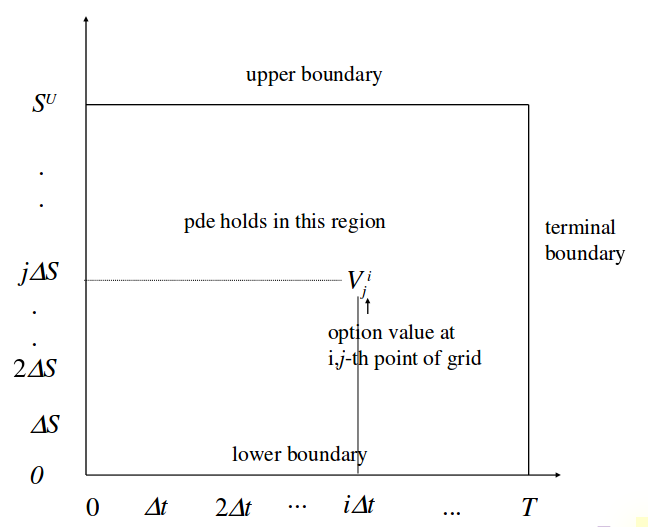
\includegraphics[width=0.5\textwidth]{grid0.png}
    \caption{ FDM grid}
\end{figure}

To work with FDM, we focus on $V^i_j$ and its neighbours:

\begin{figure}[H]
   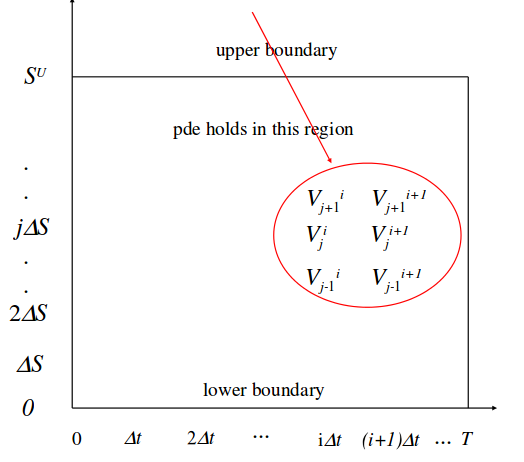
\includegraphics[width=0.5\textwidth]{grid1.png}
    \caption{ FDM grid}
\end{figure}

We know the value at maturity $T$ , so we work backward in time. Lets approximate Black-Scholes equation by difference equations:
\begin{equation}
\frac{V_j^{i+1}-V_j^i}{\Delta t} + \frac{1}{2} \sigma^2 j^2 (\Delta S)^2 \frac{V_{j+1}^{i+1}-2V_j^{i+1}-V_{j-1}^{i+1}}{(\Delta S)^2} + rj\Delta S \frac{V_{j+1}^{i+1}-V_{j-1}^{i+1}}{2\Delta S} -rV_j^i=0
\end{equation} 
where $V_j^i$ is the unknown, so by rearranging the terms we get:
\begin{equation}
V_j^i = \frac{1}{1+r\Delta t}(AV_{j+1}^{i+1}+BV_j^{i+1}+CV_{j-1}^{i+1})
\end{equation}
with 
\begin{itemize}
\item $A=(\frac{1}{2} \sigma^2 j^2+\frac{1}{2} rj)\Delta t $
\item $B=1-\sigma^2 j^2 \Delta t $
\item $C = (\frac{1}{2} \sigma^2 j^2 - \frac{1}{2}rj)\Delta t$
\end{itemize}


\textbf{Stability}\\
Explicit method is unstable, so we derive the conditions of stability by using probabilistic approach.\\
If we consider $A,B,C$ as probabilities, we require them to be positive. So, for we get for 
\begin{itemize}
\item $A$ and $C$ $\rightarrow  j > |\frac{r}{\sigma^2}|$  
\item $B \rightarrow \Delta t < \frac{1}{\sigma^2 j^2}$
\end{itemize} 
In other words, when we increase $jmax$ by 10, then $imax$ must by increased by 100.

\section{Numerical Results}
We've implemented FDM in C++ for European options and compared it with analytical solution.
\begin{figure}[H]
   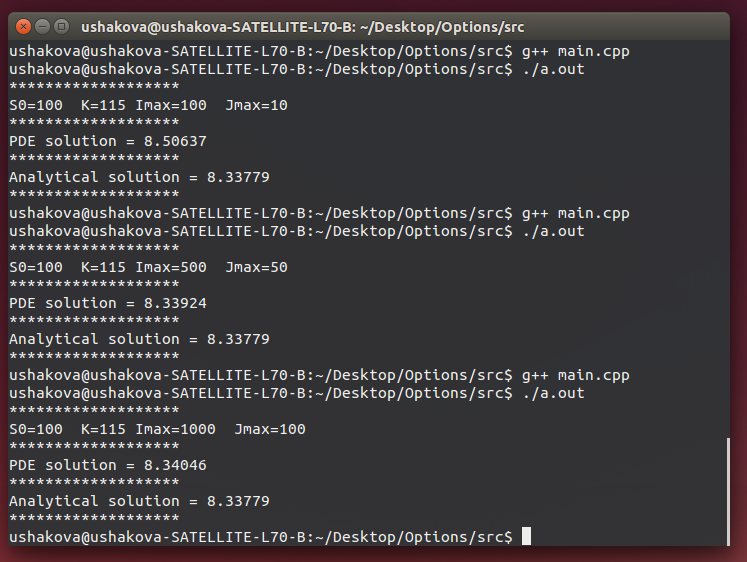
\includegraphics[width=0.7\textwidth]{fdm.png}
    \caption{ FDM and Analytical solutions}
\end{figure}

\chapter*{Conclusion}
In this project we have presented the Black-Scholes PDE. We've given the financial and stochastic background, we've also looked deeply in the Black-Scholes model and found its analytical solution.  Later we've talked about sensibility indicators called Greeks, and finally we've implemented FEM and FDM methods.\\
For the numerical results, we have particularly worked with FreeFem++ and C++. Nevertheless, the code in Feel++ is also provided (1D and 2D), however the export wasn't produced.\\
As our main goal was implementing FEM and FDM, we can conclude that each of them has its own advantages:
\begin{itemize}
\item Why use FEM?
\begin{itemize}
\item Much more accurate 
\item Lots of free libraries
\end{itemize}
\item Why use FDM?
\begin{itemize}
\item No usual boundary problems
\item Easier to implement
\end{itemize}
\end{itemize}
For further studying, we consider look deeply in models, based on other processes, like Heston or Bates model. We also look forward to master Feel++.   




\chapter*{Biblio}
\begin{enumerate}


\item Topper, J. (2005), \textit{Financial Engineering with Finite Elements} 
\item Hull, J.C. (2012), \textit{Options, futures and other derivatives} 
\item Oksendal, B (2003), \textit{Stochastic Differential Equations}
\end{enumerate}

\end{document}